\documentclass{ximera}
\title{Review of Coordinate Systems}
\begin{document}
\begin{abstract}
\end{abstract}
\maketitle

In this activity, we review coordinate systems that you've seen before, in preparation for introducing new coordinate systems in subsequent sections.

\section{Cartesian Plane}

The coordinates that you're probably most comfortable with are standard two-dimensional coordinates, also called Cartesian coordinate system on the plane.

In Cartesian coordinates, we describe a point using an $x$-coordinate and a $y$-coordinate. We write a point as $(x,y)$, where the $x$-coordinate describes the horizontal displacement of the point, and the $y$-coordinate describes the vertical displacement of the point.

\begin{image}
\begin{tikzpicture}
\draw[<->] (-1,0) -- (3,0);
\draw[<->] (0,-1) -- (0,3);
\foreach \x in  {1,2}
\draw[shift={(\x,0)},color=black] (0pt,3pt) -- (0pt,-3pt);
\foreach \x in {1,2}
\draw[shift={(\x,0)},color=black] (0pt,0pt) -- (0pt,-3pt) node[below] 
{$\x$};
\foreach \y in  {1,2}
\draw[shift={(0,\y)},color=black] (3pt,0pt) -- (-3pt,0pt);
\foreach \y in {1,2}
\draw[shift={(0,\y)},color=black] (0pt,0pt) -- (-3pt,0pt) node[left] 
{$\y$};

\foreach \x in  {1,2}
\draw[dashed] (\x,0) -- (\x,2.5);
\foreach \y in  {1,2}
\draw[dashed] (0,\y) -- (2.5,\y);

\node[draw, circle, thick, fill=black, minimum size=1mm, inner sep=0] at (2,1) {};

\node at (2.5, 1.25) {(2,1)};

\end{tikzpicture}
\end{image}

\section{Polar Coordinates}

You've also seen polar coordinates.

In polar coordinates, we describe a point with an $r$-coordinate and a $\theta$-coordinate. The $r$ coordinate gives the distance between the point and the origin, and the $\theta$-coordinate gives the angle (in radians) between the positive $x$-axis and the segment connecting the origin and the point.

We can switch between cartesian and polar coordinates using the equations
\begin{align*}
x&=r\cos\theta\\
y&=r\sin\theta
\end{align*}

\begin{image}
\begin{tikzpicture}
\draw[<->] (-1,0) -- (3,0);
\draw[<->] (0,-1) -- (0,3);

\node[draw, circle, thick, fill=black, minimum size=1mm, inner sep=0] at (2,2) {};

\draw[dashed] (0,0) -- (2,2);
\draw[black] (0.4,0) arc (0 : 45 : 0.4);

\node at (2.5, 2.25) {$(r,\theta)$};
\node at (.9, 1.1) {$r$};
\node at (0.6, 0.2) {$\theta$};

\end{tikzpicture}
\end{image}

\begin{problem}
Write the point $(r,\theta) = (5, \pi/3)$ in cartesian coordinates.
\[
(x,y) = \answer{(5/2, 5\sqrt{3}/2)}
\]
Write the point $(x,y) = (-2,2)$ in polar coordinates.
\[
(r,\theta) = \answer{(\sqrt{8}, 3\pi/4)}
\]
\end{problem}

\begin{example}
Recall that we can describe a circle of radius 2 using Cartesian points as the set of points $(x,y)$ satisfying
\[
x^2+y^2 = 4.
\]

\begin{image}
\begin{tikzpicture}
\draw[<->] (-2,0) -- (2,0);
\draw[<->] (0,-2) -- (0,2);

\draw (0,0) circle (1.5);

\node at (1.6, 0.2) {$2$};

\end{tikzpicture}
\end{image}

We would like to write describe this circle using polar coordinates.

By definition, the circle of radius $2$ centered at the origin consists of the points which are distance $2$ from the origin. Because of this, for any point on the circle, we have
\[
r = \answer{2}.
\]
There are points on the circle making every possible angle with the positive $x$-axis, so we don't need any restrictions on $\theta$. If, however, we only wanted part of the circle, we would accomplish this by restricting $\theta$.

Thus, in polar coordinates, the circle of radius $2$ centered at the origin can be described as the set of points $(r,\theta)$ such that
\[
r = 2.
\]
\end{example}

There's an important difference between Cartesian coordinates and polar coordinates: Cartesian coordinates are \emph{unique}, while polar coordinates are not. This means that, given a point $P$ in the plane, there's only one way to describe this point as $(x,y)$ using Cartesian coordinates. However, there are many ways to write the point as $(r,\theta)$, using polar coordinates.

Take, for example, the point $(1,0)$, written in Cartesian coordinates.

\begin{image}
\begin{tikzpicture}
\draw[<->] (-1,0) -- (3,0);
\draw[<->] (0,-1) -- (0,3);

\node[draw, circle, thick, fill=black, minimum size=1mm, inner sep=0] at (1.5,0) {};


\node at (1.5, 0.2) {$(1,0)$};

\end{tikzpicture}
\end{image}

This point is on the $x$-axis and is distance $1$ from the origin. Thus, perhaps the most obvious way to represent this point in polar coordinates is as $(r,\theta) = (1,0)$ (coincidentally, the same as in Cartesian coordinates). But we could also describe the angle as $2\pi$, $4\pi$, $-2\pi$, etc. So, we could also write the point in polar coordinates as $(r,\theta) = (1,2\pi)$, and so on.

Perhaps more surprisingly, we can describe this point as $(-1,\pi)$. Imagine making an angle of $\pi$ with the positive $x$-axis (so we're on the negative $x$-axis), then going backwards past the origin. This also gets you to our point. Using equivalent angles, we can also represent the point as $(-1,3\pi)$, $(-1, -\pi$, and so on.

There are some times in working with polar coordinates when we would like to be able to represent points uniquely, and in these situations, we often make restrictions
\[
\begin{array}{c}
0\leq r,\\
0\leq \theta < 2\pi.
\end{array}
\]
However, even with these restrictions, there still is a point that has multiple representations! Namely, the origin can be written as $(r,\theta) = (0,\theta)$ for any angle $\theta$.

Depending on the situation and context, different people may use different restrictions or conventions for their ranges for $r$ and $\theta$. For this reason, it's good to specify what values you're allowing, to avoid being misunderstood!

\begin{example}
Let's consider the line described in Cartesian coordinates as the set of points $(x,y)$ such that $y=x$. We'll figure out how to describe this line in polar coordinates.

\begin{image}
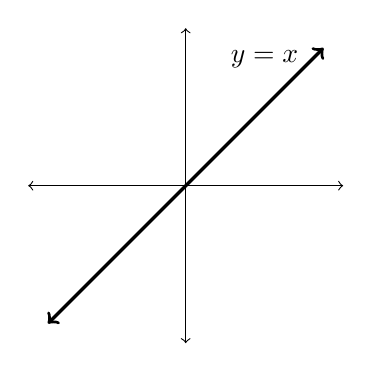
\begin{tikzpicture}
\draw[<->] (-2,0) -- (2,0);
\draw[<->] (0,-2) -- (0,2);

\draw[<->, very thick] (-1.75,-1.75) -- (1.75,1.75);

\node at (1, 1.6) {$y=x$};

\end{tikzpicture}
\end{image}

Let's restrict our polar coordinates to $0\leq r$ and $0\leq \theta <2\pi$. Perhaps your first guess is to describe the line as the points $(r,\theta)$ such that
\[
\theta = \pi/4 .
\]
Which shape does this describe?
\begin{multipleChoice}
\choice{A point.}
\choice[correct]{Half of the line.}
\choice{The whole line.}
\choice{A different line.}
\choice{A circle.}
\end{multipleChoice}

Describing the line as $\theta = \pi/4$ is a reasonable first guess, as we can see that many of the points make an angle $\pi/4$ with the positive $x$-axis. However, with the restriction that $r\geq 0$, this leaves out half of the line! In order to describe the entire line, we have a couple of options. One option would be to relax our restriction on $r$, and allow negative values as well. This would certainly give us the whole line. If, however, we would like to keep this restriction that $r\geq 0$, we could also include points with $\theta = 5\pi/4$, which will give us the other half of the line.

Which of the following describe the line $y=x$ in polar coordinates? Select all that work.
\begin{selectAll}
\choice{The points $(r,\theta)$ such that $\theta = \pi/4$, where $r\geq 0$.}
\choice[correct]{The points $(r,\theta)$ such that $\theta = \pi/4$, where $r$ can be any real number.}
\choice{The points $(r,\theta)$ such that $\theta = \pi/4$ or $\theta = -\pi/4$, where $r\geq 0$.}
\choice{The points $(r,\theta)$ such that $\theta = \pi/4$ or $\theta = -\pi/4$, where $r$ can be any real number.}
\choice[correct]{The points $(r,\theta)$ such that $\theta = \pi/4$ or $\theta = 5\pi/4$, where $r\geq 0$.}
\choice[correct]{The points $(r,\theta)$ such that $\theta = \pi/4$ or $\theta = 5\pi/4$, where $r$ can be any real number.}
\end{selectAll}

\end{example}

\begin{example}
Consider the set of points $(r,\theta)$ such that $r = 2\cos\theta$. What does this set of points look like?

It's not very clear from $r=2\cos\theta$ what shape this is describing, so let's try converting this to Cartesian coordinates, and see if we get something we recognize.

Recall that the relationship between Cartesian and polar coordinates:
\begin{align*}
x &= \answer{r\cos\theta},\\
y &= \answer{r\sin\theta}.
\end{align*}

From this, we have that $r^2 = \answer{x^2+y^2}$, in terms of $x$ and $y$, and $\cos\theta = \frac{x}{r}$. Making substitutions using these facts, we have:
\begin{align*}
r &= 2\cos\theta\\
r &= 2\frac{x}{r}\\
r^2 &= 2x\\
x^2+y^2 &= 2x\\
\end{align*}

We now have an equation solely in terms of $x$ and $y$, but maybe it isn't quite recognizable yet. But if we do a bit more algebra...
\begin{align*}
x^2 + y^2 &= 2x\\
(x^2-2x+1) + y^2 &= 1\\
(x-1)^2 + y^2 &=1
\end{align*}

Now, we can see that this is a circle of radius $1$ centered at $(1,0)$.

\begin{image}
\begin{tikzpicture}
\draw[<->] (-1,0) -- (3,0);
\draw[<->] (0,-2) -- (0,2);

\draw (1,0) circle (1);

\node at (2.2, 0.2) {$2$};

\end{tikzpicture}
\end{image}

\end{example}

\section{Linear Change of Coordinates}

In Linear Algebra, we saw how different coordinate systems arose through linear change of coordinates. You may remember this referred to as ``slanty space.''

When we write a point in Cartesian coordinates as $(x,y)$, we can think of this as a linear combination of the standard basis vectors:
\[
(x,y) = x(1,0) + y(0,1).
\]

Of course, we can just as well write a point as a linear combination of vectors from a different basis, say $(3,1)$ and $(1, -1)$. Let's call this basis $\mathfrak{B}$ For example, we can write the vector $(9,-1)$ as
\[
(9,-1) = 2(3,1)+3(1,-1).
\]
Taking the coefficients, in $\mathfrak{B}$-coordinates, we would write this point as
\[
(2,3)_{\mathfrak{B}}.
\]
Note that we write $\mathfrak{B}$ in the subscript, in order to remind us that these are $\mathfrak{B}$-coordinates, rather than standard Cartesian coordinates.

\begin{image}
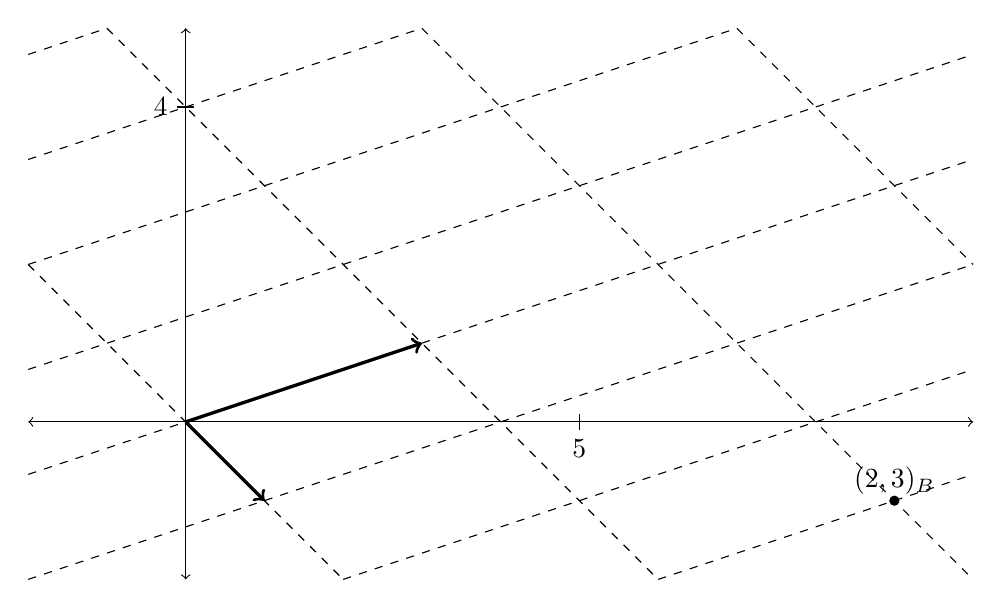
\begin{tikzpicture}
\draw[<->] (-2,0) -- (10,0);
\draw[<->] (0,-2) -- (0,5);
\foreach \x in  {5}
\draw[shift={(\x,0)},color=black] (0pt,3pt) -- (0pt,-3pt);
\foreach \x in {5}
\draw[shift={(\x,0)},color=black] (0pt,0pt) -- (0pt,-3pt) node[below] 
{$\x$};
\foreach \y in  {4}
\draw[shift={(0,\y)},color=black] (3pt,0pt) -- (-3pt,0pt);
\foreach \y in {4}
\draw[shift={(0,\y)},color=black] (0pt,0pt) -- (-3pt,0pt) node[left] 
{$\y$};

\draw[->, very thick] (0,0) -- (3,1);
\draw[->, very thick] (0,0) -- (1,-1);

\draw[dashed] (-2,-2/3) -- (10, 10/3);
\draw[dashed] (-2,-2) -- (10, 2);
\draw[dashed] (2,-2) -- (10, 2/3);
\draw[dashed] (6,-2) -- (10, -2/3);
\draw[dashed] (-2,2/3) -- (10, 14/3);
\draw[dashed] (-2,2) -- (7,5);
\draw[dashed] (-2,10/3) -- (3,5);
\draw[dashed] (-2,14/3) -- (-1,5);

\draw[dashed] (-2,2) -- (2,-2);
\draw[dashed] (-1,5) -- (6,-2);
\draw[dashed] (3,5) -- (10,-2);
\draw[dashed] (7,5) -- (10,2);

\node[draw, circle, thick, fill=black, minimum size=1mm, inner sep=0] at (9,-1) {};

\node at (9, -.75) {$(2,3)_\mathfrak{B}$};

\end{tikzpicture}
\end{image}

With linear changes of coordinates, it's easy to make a mistake and forget which coordinates you're using. Make sure to keep careful track!

\section{Three-Dimensional Coordinates}

In Linear Algebra, we also worked in three-dimensional Cartesian coordinates, $(x,y,z)$ in $\mathbb{R}^3$.

\begin{image}
\begin{tikzpicture}
\draw[<->] (-5,0) -- (5,0);
\draw[<->] (0,-5) -- (0,5);
\draw[<->] (-4,-3) -- (4,3);


\draw[dashed] (-2,-3/2) -- (1,-3/2);
\draw[dashed] (-2,-3/2) -- (-2,1/2);
\draw[dashed] (-2,1/2) -- (0,2);
\draw[dashed] (0,2) -- (3,2);
\draw[dashed] (-2,1/2) -- (1,1/2);
\draw[dashed] (3,2) -- (3,0);
\draw[dashed] (3,2) -- (1,1/2);
\draw[dashed] (1,1/2) -- (1,-3/2);
\draw[dashed] (3,0) -- (1,-3/2);

\node[draw, circle, thick, fill=black, minimum size=1mm, inner sep=0] at (1,1/2) {};

\node at (5, -.25) {$y$};
\node at (-.3, 5) {$z$};
\node at (-4, -3.25) {$x$};
\node at (1.7, .25) {$(x,y,z)$};

\end{tikzpicture}
\end{image}

It's important to remember that the $x$, $y$, and $z$ axes follow the right hand rule. That is, if you take your right hand, and point your pointer finger in the direction of the positive $x$-axis, point your middle finger in the direction of the positive $y$-axis, then your thumb points in the direction of the positive $z$-axis.

Another way to say this is that if you point the fingers of your right hand in the direction of the positive $x$-axis and curl them to point in the direction of the positive $y$-axis, your thumb points in the direction of the positive $z$-axis.


We'll often refer to the \emph{coordinate planes} in $\mathbb{R}^3$. These are the three planes we obtain by setting each of the coordinates to be zero.
\begin{image}
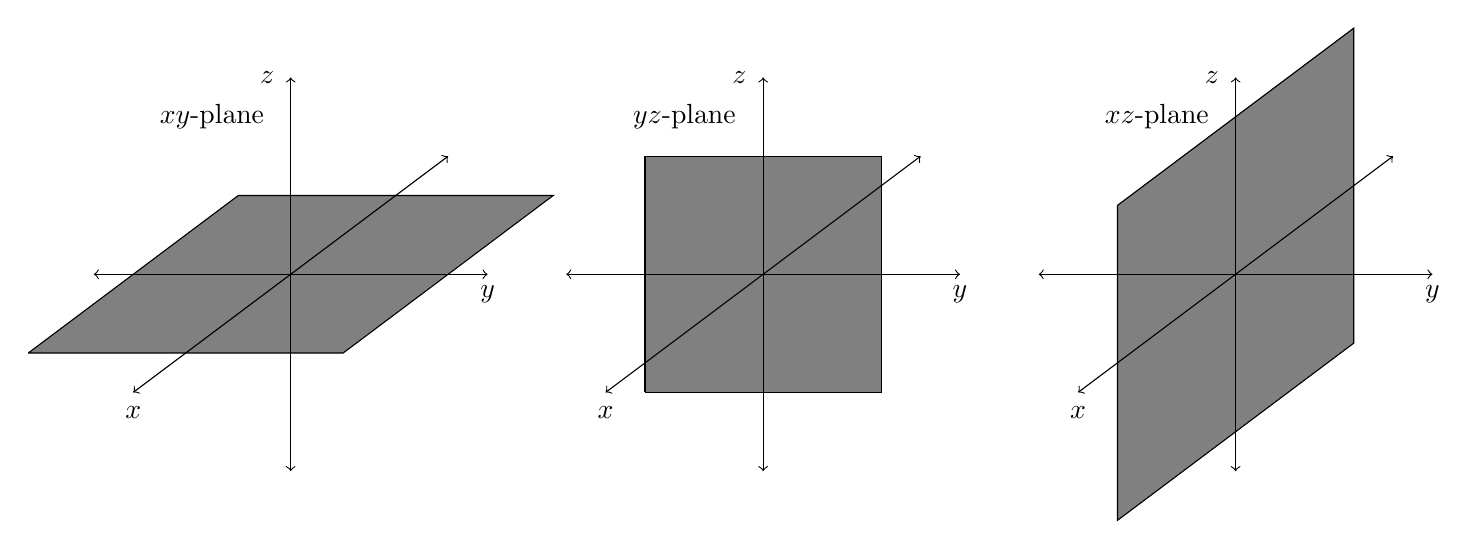
\begin{tikzpicture}

\draw[fill = gray] (-10/3,-1) -- (2/3,-1) -- (10/3, 1) -- (-2/3,1) -- (-10/3,-1);

\draw[<->] (-2.5,0) -- (2.5,0);
\draw[<->] (0,-2.5) -- (0,2.5);
\draw[<->] (-2,-1.5) -- (2,1.5);

\node at (2.5, -.25) {$y$};
\node at (-.3, 2.5) {$z$};
\node at (-2, -1.75) {$x$};

\node at (-1,2) {$xy$-plane};

\begin{scope}[shift={(6,0)}]

\draw[fill = gray] (-1.5,-1.5) -- (1.5,-1.5) -- (1.5, 1.5) -- (-1.5,1.5) -- (-1.5,-1.5);

\draw[<->] (-2.5,0) -- (2.5,0);
\draw[<->] (0,-2.5) -- (0,2.5);
\draw[<->] (-2,-1.5) -- (2,1.5);

\node at (2.5, -.25) {$y$};
\node at (-.3, 2.5) {$z$};
\node at (-2, -1.75) {$x$};

\node at (-1,2) {$yz$-plane};

\end{scope}

\begin{scope}[shift={(12,0)}]

\draw[fill = gray] (-1.5,7/8) -- (-1.5,-25/8) -- (1.5, -7/8) -- (1.5,25/8) -- (-1.5,7/8);

\draw[<->] (-2.5,0) -- (2.5,0);
\draw[<->] (0,-2.5) -- (0,2.5);
\draw[<->] (-2,-1.5) -- (2,1.5);

\node at (2.5, -.25) {$y$};
\node at (-.3, 2.5) {$z$};
\node at (-2, -1.75) {$x$};

\node at (-1,2) {$xz$-plane};

\end{scope}

\end{tikzpicture}
\end{image}

More precisely, the $xy$-plane is the set of points $(x,y,z)$ such that $z = 0$, the $yz$-plane is the set of points such that $x = 0$, and the $xz$-plane is the set of points such that $y = 0$.

Similarly to in the plane, we can describe sets of points in $\mathbb{R}^3$ using equations.

\begin{example}
The set of points $(x,y,z)$ such that $x^2+y^2+z^2 = 1$ is the sphere of radius 1 centered at the origin in $\mathbb{R}^3$.

\begin{image}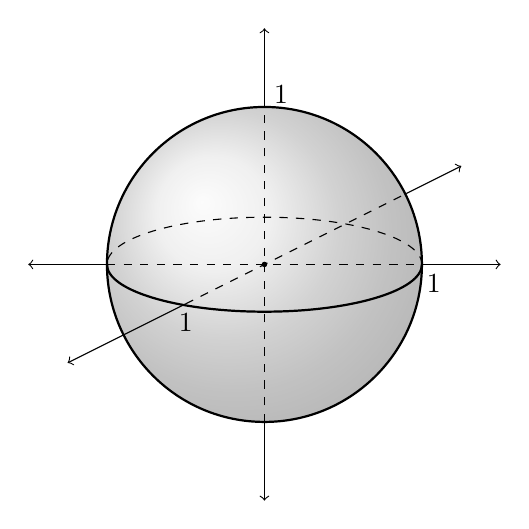
\begin{tikzpicture}
  \shade[ball color = gray!40, opacity = 0.4] (0,0) circle (2cm);
  \draw[thick] (0,0) circle (2cm);
  \draw[thick] (-2,0) arc (180:360:2 and 0.6);
  \draw[dashed] (2,0) arc (0:180:2 and 0.6);
  \fill[fill=black] (0,0) circle (1pt);
  
  \draw[<-] (-3, 0) -- (-2,0);
  \draw[dashed ] (-2,0 ) -- (2,0) node[below, xshift=1ex] 
{$1$};
  \draw[->] (2,0) -- (3,0);
  \draw[<-] (0, -3) -- (0,-2);
  \draw[dashed] (0,-2 ) -- (0,2) node[right, yshift = 1ex] 
{$1$};
  \draw[->] (0,2) -- (0,3);
  \draw[<-] (-2.5, -1.25) -- (-1,-0.5);
  \draw[dashed] (-1,-0.5) node[below] 
{$1$} -- (1.8, 0.9);
  \draw[->] (1.8, 0.9) -- (2.5, 1.25);
\end{tikzpicture}\end{image}


\end{example}

\section{Conclusion}

In this activity, we reviewed coordinate systems that you've seen before: standard two-dimensional coordinates, polar coordinates, coordinates with respect to a given set of basis vectors, and three-dimensional coordinates.

\end{document}
